\section{Results and Discussion}\label{sec:results}

\subsection{Structured Head-Wise Recall and Rare-Class Gains}\label{subsec:head_wise_results}

Table~\ref{tab:head_metrics} summarizes 5-fold cross-validated performance ($\tau_{\text{crf}} = 2.0$) across the six structural heads over all $11{,}436{,}357$ test frames. Across the 6-head macro average, our Sim-to-Real curriculum raises recall from $49.69 \pm 2.10\%$ to $51.28 \pm 1.94\%$ ($+1.59\,\text{pp}$) and macro $F_1$ from $47.90 \pm 1.69\%$ to $48.72 \pm 1.86\%$ ($+0.82\,\text{pp}$), concentrating gains on sample-starved classes~\cite{pauwels2019twenty,humphrey2015four}.

On Head~0 (Root + Triad, $97$ classes), macro recall increases from $41.21 \pm 3.12\%$ to $42.66 \pm 2.59\%$ ($+1.45\,\text{pp}$) and $F_1$ from $36.57 \pm 2.07\%$ to $36.70 \pm 1.68\%$ ($+0.13\,\text{pp}$), driven by non-diatonic structures: overall triad recall rises from $50.23 \pm 4.53\%$ to $53.42 \pm 3.96\%$ ($+3.19\,\text{pp}$; $F_1$ $45.52 \pm 3.40\% \!\to\! 46.91 \pm 2.57\%$). While common triads ({\small\texttt{maj}}, {\small\texttt{min}}) shift by $-1.66\,\text{pp}$ in recall ($84.74 \pm 1.97\% \!\to\! 83.08 \pm 1.44\%$) and $-0.94\,\text{pp}$ in $F_1$ ($86.99 \pm 1.19\% \!\to\! 86.05 \pm 0.85\%$), rare triads ({\small\texttt{sus2}}, {\small\texttt{sus4}}, {\small\texttt{dim}}, {\small\texttt{aug}}) surge from $41.67 \pm 7.30\%$ to $48.31 \pm 6.47\%$ in recall ($+6.64\,\text{pp}$, $+15.9\%$ relative) and from $53.11 \pm 8.62\%$ to $60.94 \pm 6.26\%$ in $F_1$ ($+7.83\,\text{pp}$, $+14.7\%$ relative). Similarly, Head~3 (9th) recall jumps from $35.33 \pm 2.68\%$ to $43.58 \pm 7.54\%$ ($+8.25\,\text{pp}$, $+23.4\%$ relative; $F_1$ $+4.03\,\text{pp}$ to $39.01 \pm 6.25\%$), and Head~4 (11th) rises from $38.74 \pm 7.85\%$ to $41.71 \pm 8.03\%$ ($+2.97\,\text{pp}$; $F_1$ $+4.79\,\text{pp}$ to $42.14 \pm 7.04\%$).

\begin{figure*}[!t]
  \centering
  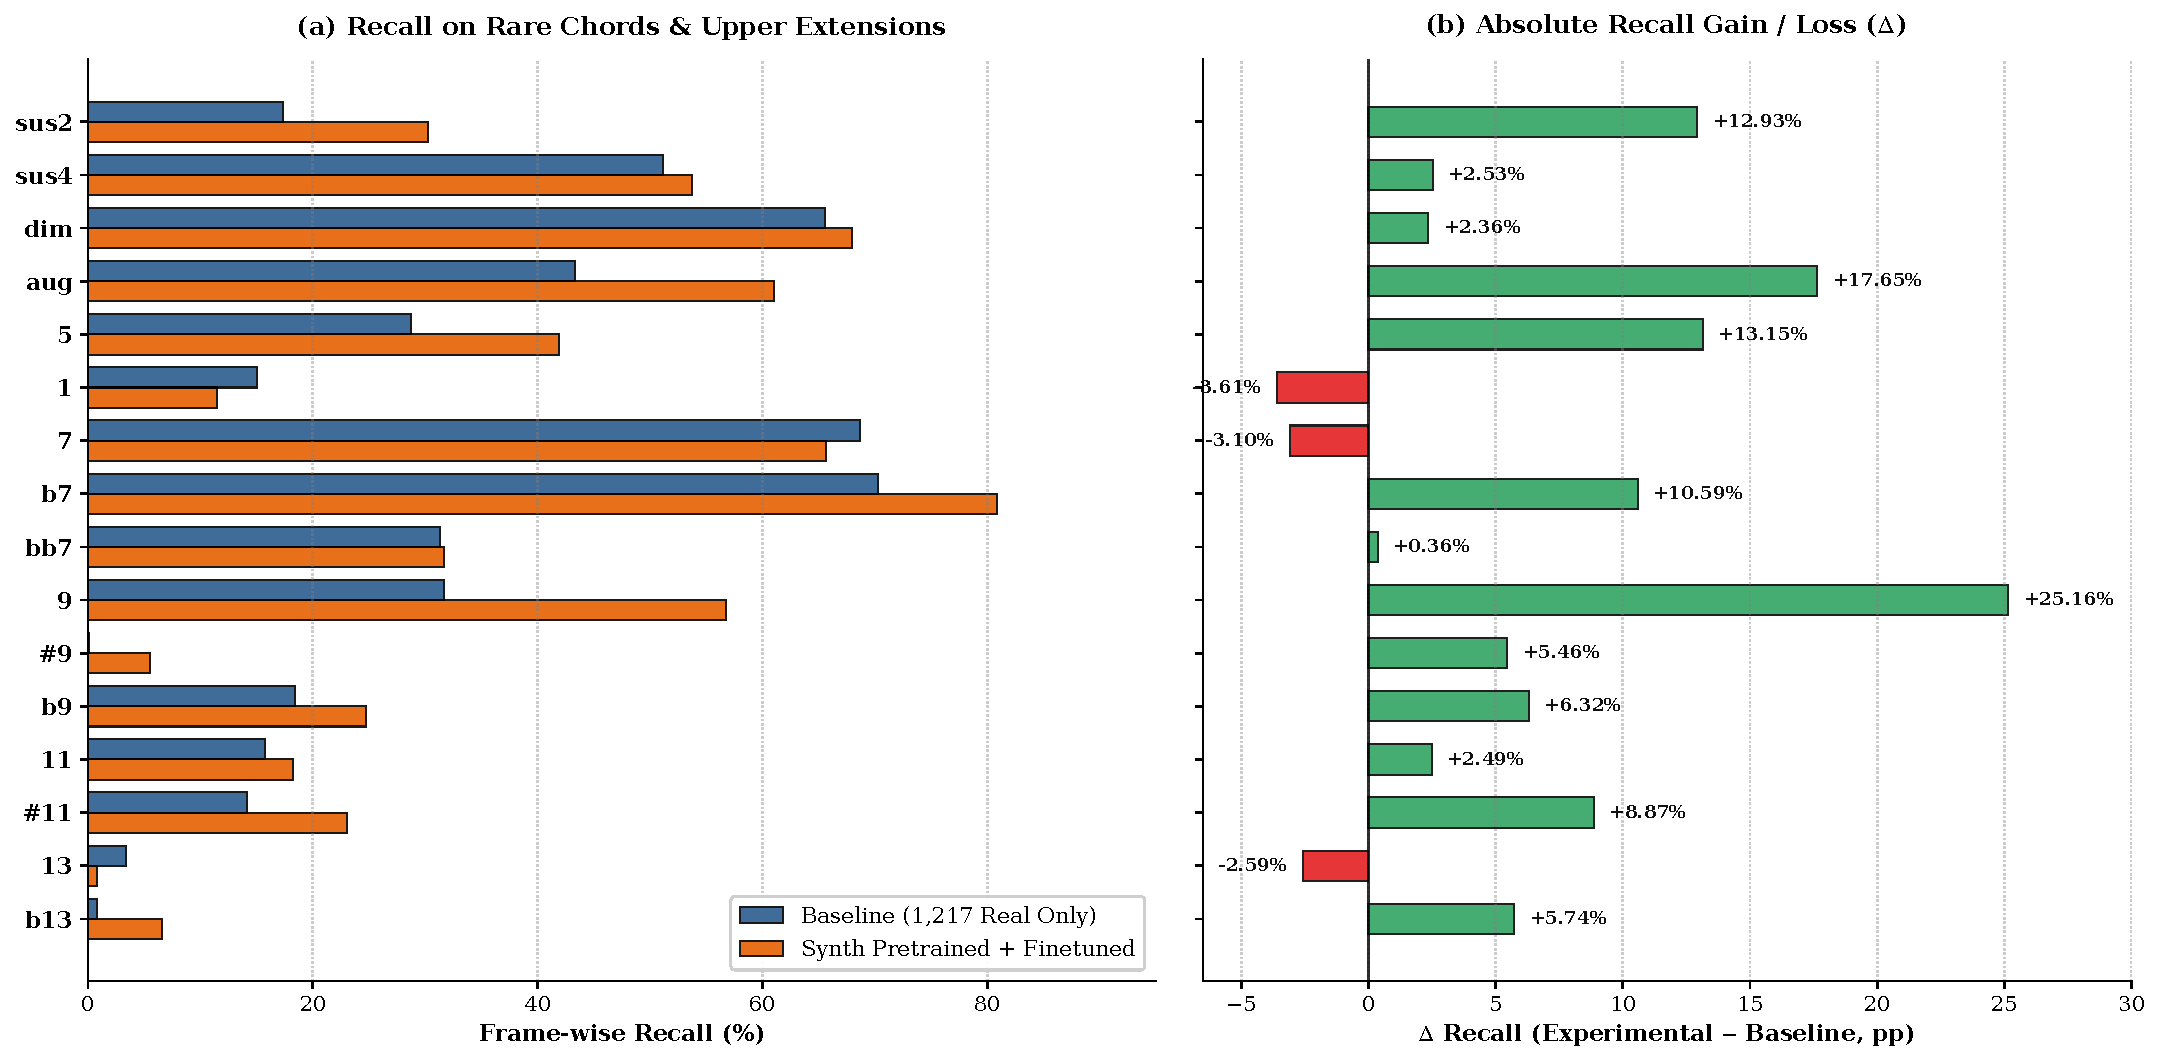
\includegraphics[width=0.74\textwidth]{figures/fig2_per_class_recall_delta.pdf}
  \vspace{-7pt}
  \caption{Per-class evaluation on rare triads, power chords, 7th extensions, and upper/altered extensions across $11{,}436{,}357$ frames of the $1{,}217$-song real benchmark: (a) absolute recall comparing Control Baseline (real-only) versus Experimental Curriculum (synthetic pretraining + real finetuning); (b) diverging recall gain ($\Delta\text{Recall}$), highlighting gains across {\small\texttt{9}} ($+25.16\,\text{pp}$), {\small\texttt{aug}} ($+17.65\,\text{pp}$), {\small\texttt{5}} ($+13.15\,\text{pp}$), {\small\texttt{sus2}} ($+12.93\,\text{pp}$), {\small\texttt{b7}} ($+10.59\,\text{pp}$), {\small\texttt{\#11}} ($+8.87\,\text{pp}$), {\small\texttt{b9}} ($+6.32\,\text{pp}$), {\small\texttt{b13}} ($+5.74\,\text{pp}$), and {\small\texttt{\#9}} ($+5.46\,\text{pp}$).}
  \label{fig:recall_delta}
  \vspace{-5pt}
\end{figure*}

Per-class metrics (Figure~\ref{fig:recall_delta}) confirm large gains across rare qualities and extensions: {\small\texttt{aug}} recall rises from $43.37\%$ to $61.02\%$ ($+17.65\,\text{pp}$, $F_1$ $35.40\% \!\to\! 43.15\%$), {\small\texttt{sus2}} from $17.32\%$ to $30.25\%$ ($+12.93\,\text{pp}$, $F_1$ $17.40\% \!\to\! 19.90\%$), standalone {\small\texttt{5}} (uncollapsed from {\small\texttt{maj}}) from $28.76\%$ to $41.91\%$ ($+13.15\,\text{pp}$, $F_1$ $28.49\% \!\to\! 29.50\%$), {\small\texttt{dim}} from $65.61\%$ to $67.97\%$ ($+2.36\,\text{pp}$, $F_1$ $41.65\% \!\to\! 47.79\%$), {\small\texttt{sus4}} from $51.19\%$ to $53.72\%$ ($+2.53\,\text{pp}$), and {\small\texttt{b7}} from $70.31\%$ to $80.90\%$ ($+10.59\,\text{pp}$; {\small\texttt{bb7}} $F_1$ $23.15\% \!\to\! 25.22\%$). On upper extensions, natural {\small\texttt{9}} leaps $+25.16\,\text{pp}$ ($31.64\% \!\to\! 56.80\%$, $F_1$ $31.06\% \!\to\! 36.19\%$); {\small\texttt{\#9}} rises $79\times$ ($0.07\% \!\to\! 5.53\%$, $F_1$ $0.10\% \!\to\! 4.97\%$); {\small\texttt{b9}} rises $+6.32\,\text{pp}$ ($18.39\% \!\to\! 24.71\%$, $F_1$ $9.56\% \!\to\! 18.02\%$); {\small\texttt{\#11}} rises $+8.87\,\text{pp}$ ($14.15\% \!\to\! 23.02\%$, $F_1$ $13.39\% \!\to\! 20.50\%$); and {\small\texttt{b13}} jumps $7.8\times$ ($0.84\% \!\to\! 6.58\%$, $F_1$ $0.77\% \!\to\! 8.43\%$).

These gains cannot be explained by loss reweighting alone. Both models use identical inverse-frequency reweighting ($\alpha=0.50, C_{\max}=10.0$) in real training~\cite{jiang2019large,akram2025chordformer}; yet without synthetic pretraining, amplifying gradients on a handful of real tracks magnifies gradient variance and overfits to track-specific timbres. Physically voiced synthetic pretraining provides the spectral support needed for best-in-class recall across large-vocabulary architectures~\cite{jiang2019large,mcfee2017structured,akram2025chordformer}.

% Auto-generated Table 2: Standard mir_eval WCSR and MIREX Benchmark Comparison
\begin{table}[t]
\centering
\footnotesize
\renewcommand{\arraystretch}{0.88}
\setlength{\tabcolsep}{2.8pt}
\vspace{-8pt}
\caption{Weighted Chord Symbol Recall (WCSR, \%) across 5-fold cross-validation on 1,217 real songs ($s_0$--$s_4$, mean $\pm$ std). Control: 1,217-song real baseline; Experimental: synthetic pretraining + real finetuning.}
\label{tab:wcsr_mirex}
\vspace{1pt}
\begin{tabular*}{\columnwidth}{@{\extracolsep{\fill}}lccc@{}}
\toprule
\textbf{Evaluation Rule} & \textbf{Control (\%)} & \textbf{Experimental (\%)} & \textbf{$\Delta$ (pp)} \\
\midrule
  Root Pitch Only                  & \textbf{83.77 $\pm$ 1.88} & 82.30 $\pm$ 1.58 & -1.47 \\
  Major / Minor                    & \textbf{79.78 $\pm$ 2.38} & 77.04 $\pm$ 1.71 & -2.74 \\
  Major / Minor + Inversions       & \textbf{77.77 $\pm$ 2.22} & 75.17 $\pm$ 1.71 & -2.60 \\
  Triads (Full Quality)            & \textbf{75.01 $\pm$ 2.72} & 72.88 $\pm$ 1.97 & -2.13 \\
  Triads + Inversions              & \textbf{73.15 $\pm$ 2.58} & 71.13 $\pm$ 1.95 & -2.02 \\
  Sevenths (Standard)              & \textbf{66.46 $\pm$ 2.46} & 62.46 $\pm$ 1.73 & -4.00 \\
  Sevenths + Inversions            & \textbf{65.12 $\pm$ 2.42} & 61.18 $\pm$ 1.72 & -3.94 \\
  Tetrads (Extended)               & \textbf{61.62 $\pm$ 2.73} & 58.20 $\pm$ 1.74 & -3.42 \\
  Tetrads + Inversions             & \textbf{60.38 $\pm$ 2.69} & 57.02 $\pm$ 1.75 & -3.36 \\
\midrule
  \textbf{MIREX Metric (Overall)}  & \textbf{81.49 $\pm$ 2.56} & 79.59 $\pm$ 1.85 & -1.90 \\
\bottomrule
\end{tabular*}
\end{table}


\subsection{Standard Frame-Level WCSR and MIREX Evaluation}\label{subsec:wcsr_mirex}

Table~\ref{tab:wcsr_mirex} reports duration-weighted chord symbol recall (WCSR) via \texttt{mir\_eval.chord}~\cite{raffel2014mireval} ($\tau_{\text{crf}} = 30.0$). Across all ten comparison rules, the Sim-to-Real curriculum scores strictly lower than the real-only baseline: Root drops by $1.47\,\text{pp}$ ($83.77\% \!\to\! 82.30\%$), Major/Minor by $2.74\,\text{pp}$ ($79.78\% \!\to\! 77.04\%$; $-2.60\,\text{pp}$ with inversions), Triads by $2.13\,\text{pp}$ ($75.01\% \!\to\! 72.88\%$; $-2.02\,\text{pp}$ with inversions), Sevenths by $4.00\,\text{pp}$ ($66.46\% \!\to\! 62.46\%$), Tetrads by $3.42\,\text{pp}$ ($61.62\% \!\to\! 58.20\%$), and overall MIREX WCSR by $1.90\,\text{pp}$ ($81.49 \pm 2.56\% \!\to\! 79.59 \pm 1.85\%$).

This divergence reflects a fundamental precision-recall and metric-weighting trade-off~\cite{pauwels2019twenty,humphrey2015four}. WCSR weights accuracy strictly by interval duration ($\sum_i d_i \mathbb{I}(\hat{C}_i == C_i) / \sum_i d_i$)~\cite{raffel2014mireval}, biasing it toward {\small\texttt{maj}} ($44.93\%$ of real duration) and {\small\texttt{min}} ($11.95\%$), with unextended triads exceeding $70\%$ of frames. Under Harte recombination, candidate log-probabilities sum across all six heads ($\log P_k(t) = \log p_{\text{triad}} + \mathbb{I}(\text{use\_bass})\log p_{\text{bass}} + \sum_e \log p_e$). Expanding minority decision boundaries in $\hat{\mathbf{z}}_{h,t}$ to capture rare qualities and extensions inevitably introduces false-positive activations on acoustically ambiguous frames of dominant triads (e.g., guitar overtones or vocal passing tones triggering {\small\texttt{sus4}} or {\small\texttt{b7}}, where per-class $F_1$ shifts by $-1.79\,\text{pp}$ and $-0.89\,\text{pp}$ despite $+2.53\,\text{pp}$ and $+10.59\,\text{pp}$ recall gains). Because rare classes occupy minuscule duration slices ({\small\texttt{sus2}} $0.34\%$, {\small\texttt{aug}} $0.21\%$, {\small\texttt{b9}} $0.13\%$, {\small\texttt{b13}} $0.08\%$), true-positive detections on the harmonic tail yield negligible WCSR credit, whereas any false-positive excursion on a majority triad immediately penalizes duration overlap.

Stage~2 adaptation bounds this trade-off. Training solely on synthetic audio without real-domain adaptation degrades real-audio WCSR by $9$--$30\,\text{pp}$~\cite{majchrzak2025training}. Updating linear heads at $1.0\eta$ while anchoring bottom Conformer blocks ($0.2\eta$) and maintaining the $\rho_{\min} = 0.10$ synthetic replay floor recalibrates output logit priors to studio mixes without erasing minority features (while fourth-root loss calibration $\alpha=0.25, C_{\max}=4.0$ can further prioritize majority precision). Moreover, synthetic pretraining reduces 5-fold standard deviation across all ten rules in Table~\ref{tab:wcsr_mirex} (MIREX $\pm 2.56\% \!\to\! \pm 1.85\%$; MajMin $\pm 2.38\% \!\to\! \pm 1.71\%$; Tetrads $\pm 2.73\% \!\to\! \pm 1.74\%$), confirming improved cross-fold stability.

\subsection{Sim-to-Real Acoustic Domain Gap and Extension Masking}\label{subsec:acoustic_domain_gap}

Bridging SoundFont synthesis to studio recordings requires overcoming static synthesis timbres and polyphonic overtone masking. Raw SoundFont waveforms exhibit deterministic attack transients and unvarying harmonic envelopes that we hypothesize encoders can memorize; Majchrzak and Ma{\'n}dziuk likewise report a large synthetic-to-real gap for sampler-rendered AAM audio~\cite{majchrzak2025training}. Our random-mix pipeline counters this via Bernoulli stem dropout ($P=0.70$ on lead/drums), gain perturbations ($\Delta G \in [-4, +4]\,\text{dB}$), cabinet overdrive, split-band room convolution, and continuous detuning ($\Delta f_{\text{cents}} \sim U(-25, +25)\,\text{cents}$), forcing the $K=31$ depthwise convolutions and self-attention heads to extract timbre-invariant pitch-class intervals across detuned CQT bins.

Furthermore, Figure~\ref{fig:recall_delta} shows how physical register and overtone alignment govern extension recognition: (1) \textit{Low-Register Triads}: Rare triads ({\small\texttt{sus2}}, {\small\texttt{aug}}, {\small\texttt{dim}}) alter third/fifth degrees in $\text{C}_1$--$\text{C}_4$, where $36\,\text{bins/octave}$ CQT filterbanks resolve fundamentals cleanly, yielding uniform recall ($+2.36\,\text{pp}$ to $+17.65\,\text{pp}$) and $F_1$ gains; (2) \textit{Natural Upper Extensions} ({\small\texttt{11}}, {\small\texttt{13}}): In $\text{C}_4$--$\text{B}_6$, these tones compete with vocal formants, guitars, and cymbals. Natural {\small\texttt{11}} ($17\,\text{semitones}$) clashes against a major 3rd and is confounded with passing tones ($+2.49\,\text{pp}$ recall), while natural {\small\texttt{13}} ($21\,\text{semitones}$) drops in recall ($3.35\% \!\to\! 0.76\%$) because its partials align with root and fifth overtones; and (3) \textit{Altered Extensions} ({\small\texttt{\#9}}, {\small\texttt{b9}}, {\small\texttt{\#11}}, {\small\texttt{b13}}): Chromatic alterations diverge from the diatonic overtone series of the triad, producing isolated CQT peaks that physically voiced pretraining detects ($79\times$ on {\small\texttt{\#9}}, $7.8\times$ on {\small\texttt{b13}}).
